\documentclass[12pt]{article}
\usepackage[utf8]{inputenc}
\usepackage[czech]{babel}
\usepackage{enumitem}
\usepackage{caption}
\usepackage{url}
\usepackage{graphicx}
\usepackage{footnote}
\makesavenoteenv{tabular}

\usepackage{float}

\begin{document}

\begin{center}
\bf Semestrální projekt MI-PAP 2015/2016:\\[5mm]
    Modelování částic\\[5mm]
       Miroslav Brabenec\\
       Jan Nováček\\[2mm]
magisterské studium, FIT ČVUT, Thákurova 9, 160 00 Praha 6\\[2mm]
\today
\end{center}
%
%
%
% Co má být ve zprávě: https://edux.fit.cvut.cz/courses/MI-PAP/labs/technicka_zprava
%
%
\section{Definice problému, popis sekvenčního algoritmu a jeho implementace}

\subsection{Definice problému}
Implementujte tento algoritmus (viz \url{http://www.browndeertechnology.com/docs/BDT_OpenCL_Tutorial_NBody-rev3.html#algorithm}) a upravte ho takto:

\begin{enumerate}
\item	částice při nárazu provedou pružný odraz a
\item	každá částice má svůj náboj
\end{enumerate}

Úkol: doplňte o možnost vizualizace (alespoň exportem dat v daných časových okamžicích ve formátu vhodném pro vizualizaci v nástroji třetích stran např. ) 

\subsection{Popis sekvenčního algoritmu}
Simulátor načte nastavení simulace ze vstupního souboru, z toho nainicializuje hodnoty a spustí simulaci.

V každém kroku simulace se vypočítává nová pozice každé částice, nová pozice záleží na vlastnostech dané částice a také na vlivu ostatních částic na tuto částici.

Simulace končí po provedení zadaného počtu kroků.

Vizualizovat simulaci lze dvěma způsoby.
První umožňuje sledovat průběh simulace jako animaci přímo za běhu, k tomu byla využita knihovna CImg.
Druhý způsob využívá možností programu gnuplot,
simulátor vytvoří zdrojový soubor pro vizualizaci v gnuplotu a zároveň vytvoří soubor se zdrojovými daty, která se mají vykreslit.

\subsection{Sekvenční implementace}

Bylo implementováno několik sekvenčních variant, lišících se v míře ruční vektorizace struktur použitých v algoritmu.

První varianta (V1) používá pouze automatickou optimalizaci, nepoužívá žádné SSE instrukce ani ručně vytvořené vektory.

V druhé variantě (V2) je automatická optimalizace a vektorizace. % a SSE instrukce pro výpočet ${\frac{1}{\sqrt{x}}}$.

Ve třetí variantě (V3) je automatická optimalizace a vektorizace, SSE datové typy~\_\_m128 a SSE in\-struk\-ce pro výpočet ${\frac{1}{\sqrt{x}}}$.

Porovnání rychlostí jednotlivých sekvenčních implementací je v tabulce níže.

\begin{center}
\begin{tabular}{c | c | c | c | c}
\textbf{Počet částic} & \textbf{Počet kroků sim.}  & \textbf{V1} & \textbf{V2} & \textbf{V3} \\ \hline \hline
1024 & 50 000 & 760.19s & 149.38s & 97.98s \\ \hline
512 & 400 000 & 1526.06s & 357.50s & 202.17s \\ \hline
4096 & 5 000 & 1215.77s & 207.57s & 153.81s \\ \hline
8192 & 1 500 & 1459.20s & 242.25s & 184.60s \\ \hline
\end{tabular}
\captionof{table}{Časy sekvenčních implementací}
\end{center}

\section{Popis paralelního algoritmu a jeho implementace v OpenMP}
%Popis případných úprav algoritmu a jeho implementace, včetně volby datových struktur
Paralelizace algoritmu proběhla tak, že se v každém kroku simulace rozdělí částice mezi zadaný počet vláken, paralelně se tedy počítají nové pozice částic.
Rozdělení částic mezi vlákna bylo ponecháno na OpenMP.

% Zda byla využita vektorizace (popř. proč jí nemožno využít)
\subsection{Vektorizace}

V prog\-ramu byla nej\-prve pou\-žita au\-toma\-tická vekto\-ri\-za\-ce (-O3 -mavx).
Její výsledek měl na rychlost výpočtu minimální vliv. Výrazné zrychlení nastalo, až po přidání přepínače -ffast-math.
Díky tomuto přepínači mohl kompilátor použít vektorové instrukce pro výpočet ${\frac{1}{\sqrt{x}}}$. 

V další fázi byl kód ručně upraven, tak aby bylo možné využít vektorové instrukce, které dokáží počítat paralelně několik hodnot ${\frac{1}{\sqrt{x}}}$.
Zde byly částice rozděleny do chunků po 4 a v každém kroku se počítá ovlivnění částice chunkem částic.
Tato varianta vykazovala další zrychlení cca o 33\% oproti předchozí variantě (-O3 -mavx -ffast-math).

% Popis optimalizací pro dosažení lineárního zrychlení
\subsection{Optimalizace}
Pro ruční vektorizaci byly využity technologie obsažené již v SSE2 (datový typ \_\_m128). Dalšího zrychlení by bylo možno dosáhnout při použití novějších vektorových instrukcí.
Ty by měly umožňovat tvorbu chunků o velikosti 8, případně 16.
Dále by také bylo možno upravit kód, tak aby docházelo k počítání vzdálenosti mezi částicemi pouze jednou.
Momentálně se počítá vzdálenost mezi částicemi A a B dvakrát, jednou z pohledu částice A a jednou z pohledu částice B.

\subsection{Vstupní data}
Pro měření jsme vytvořili 4 vzorky dat. Vzorky dat se lišily v počtu částic a počtu kroků simulace.
Všechny vzorky byly srovnatelné co se týče výpočetní náročnosti. Výpočetní náročnost lze spočítat jako ${N = P^2 \times S}$, kde P = počet částic a S = počet kroků.
Efektivita paralelního výpočtu se zlepšuje s rostoucím počtem částic.

\begin{center}
\begin{tabular}{c | c | c }
\textbf{Počet částic} & \textbf{Počet kroků sim.}  & \textbf{Výpočetní náročnost}\footnote{Spočítáno podle vzorce ${\frac{P^2 \times S}{10^9}}$, kde P = počet částic a S = počet kroků} \\ \hline \hline
1024 & 50 000 & 52,428 \\ \hline
512 & 400 000 & 104,857 \\ \hline
4096 & 5 000 & 83,804 \\ \hline
8192 & 1 500 & 100,663 \\ \hline
\end{tabular}
\captionof{table}{Vzorky použité pro srovnání sekvenčních implementací}
\end{center}

Po naměření časů sekvenčních implementací bez vektorizace a s vektorizací jsme usoudili, že pro měření paralelních implementací zvýšíme výpočetní náročnost úloh.
Samotná vektorizace zrychlila sekvenční část mnohonásobně - simulace běžící sekvenčně bez vektorizace téměř 25 minut trvala s vektorizací 3-4 minuty.

\begin{center}
\begin{tabular}{c | c | c | c}
\textbf{Měření} & \textbf{Počet částic} & \textbf{Počet kroků sim.} & \textbf{Výpočetní náročnost} \\ \hline \hline
1 & 1024 & 150 000 & 157,284 \\ \hline
2 & 512 & 1 200 000 & 314,571 \\ \hline
3 & 4096 & 15 000 & 251,412 \\ \hline
4 & 8192 & 4 500 & 301.989 \\ \hline
\end{tabular}
\captionof{table}{Nové zadání pro měření paralelního zrychlení}
\end{center}

% Tabulkově a případně graficky zpracované naměřené hodnoty časové složitosti měřených instancí běhu (optimalizované implementace) programu s popisem instancí dat
\section{Naměřené výsledky a vyhod\-noce\-ní pro O\-pen\-MP}
K měření výkonu paralelní implementace bylo původní zadání pozměněno tak, aby bylo výpočetně náročnější, viz předchozí tabulka.
U každého měření je uvedena tabulka s počtem vláken a časem výpočtu ve vteřinách, informace z tabulky jsou dále vyneseny do grafu.
Na konci měření k jednotlivým variantám jsou grafy s paralelním zrychlením.
Na konci sekce je porovnání a vyhodnocení měření.

\subsection{Měření pro variantu 2}
Varianta 2 využívá automatické vektorizace. % (-O3) a SSE instrukce pro výpočet ${\frac{1}{\sqrt{x}}}$.
\begin{table}[H]
\parbox{.45\linewidth}{
%
% 1. měření
%
\begin{center}
\begin{tabular}{ c | c }
\textbf{Počet vláken} & \textbf{Naměřený čas} \\ \hline \hline 
1 & 448.140625s \\ \hline
2 & 422.681641s \\ \hline
4 & 269.634277s \\ \hline
8 & 253.593750s \\ \hline
12 & 220.276367s \\ \hline
16 & 188.523438s \\ \hline
24 & 188.625000s \\ \hline
\end{tabular}
\captionof{table}{Časy 1. měření}
\end{center}
}
\hfill
\parbox{.45\linewidth}{
%
% 2. měření
%
\begin{center}
\begin{tabular}{ c | c }
\textbf{Počet vláken} & \textbf{Naměřený čas} \\ \hline \hline 
1 & 1066.172363s \\ \hline
2 & 1004.078125s \\ \hline
4 & 773.147461s \\ \hline
8 & 765.203125s \\ \hline
12 & 807.484375s \\ \hline
16 & 782.453125s \\ \hline
24 & 640.501953s \\ \hline
\end{tabular}
\captionof{table}{Časy 2. měření}
\end{center}
}
\end{table}
\begin{table}[H]
\parbox{.45\linewidth}{
%
% 3. měření
%
\begin{center}
\begin{tabular}{ c | c }
\textbf{Počet vláken} & \textbf{Naměřený čas} \\ \hline \hline 
1 & 621.765625s \\ \hline
2 & 364.220703s \\ \hline
4 & 185.841797s \\ \hline
8 & 109.250000s \\ \hline
12 & 101.171875s \\ \hline
16 & 84.234375s \\ \hline
24 & 74.109375s \\ \hline
\end{tabular}
\captionof{table}{Časy 3. měření}
\end{center}
}
\hfill
\parbox{.45\linewidth}{
%
% 4. měření
%
\begin{center}
\begin{tabular}{ c | c }
\textbf{Počet vláken} & \textbf{Naměřený čas} \\ \hline \hline 
1 & 720.630859s \\ \hline
2 & 372.531250s \\ \hline
4 & 190.187500s \\ \hline
8 & 92.015625s \\ \hline
12 & 84.015625s \\ \hline
16 & 76.273438s \\ \hline
24 & 51.625000s \\ \hline
\end{tabular}
\captionof{table}{Časy 4. měření}
\end{center}
}
\end{table}

\begin{figure}[H]
  \begin{center}
     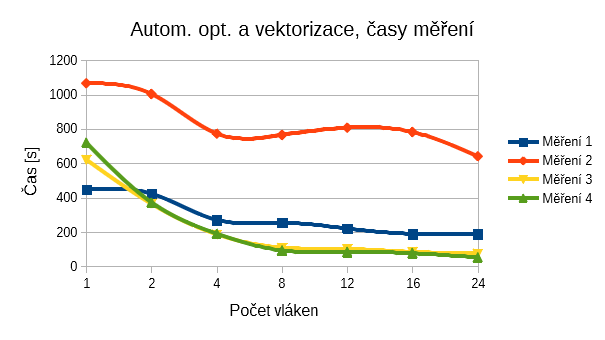
\includegraphics[width=12cm]{images/sdruzene/openmp/autotime.png}
    \caption{Výsledky měření} 
  \end{center}
\end{figure}

Z naměřených výsledků lze usoudit, že paralelizace algoritmu zredukuje výpočetní čas znatelně, až 14${\times}$.
Z měření je vidět, že čím více částic bylo v simulaci, tím vyššího zrychlení bylo dosaženo.
Vyšší počet kroků simulace naopak zrychlení spíš srážel, někdy dokonce zpomaloval.
Lineárního zrychlení dosaženo nebylo, jak je vidět z následujících grafů.

\begin{figure}[H]
  \begin{center}
     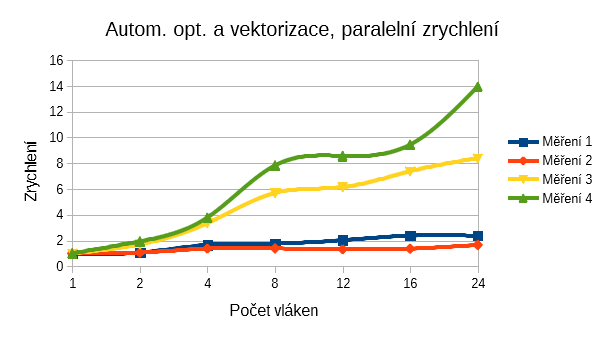
\includegraphics[width=12cm]{images/sdruzene/openmp/autoacc.png}
    \caption{Paralelní zrychlení} 
  \end{center}
\end{figure}

\subsection{Měření pro variantu 3}
Ve třetí variantě (V3) je automatická optimalizace, automatická a ruční vektorizace, mj. SSE datové typy~\_\_m128 a SSE in\-struk\-ce pro výpočet ${\frac{1}{\sqrt{x}}}$.
\begin{table}[H]
\parbox{.45\linewidth}{
%
% 1. měření
%
\begin{center}
\begin{tabular}{ c | c }
\textbf{Počet vláken} & \textbf{Naměřený čas} \\ \hline \hline 
1 & 292.988647s \\ \hline
2 & 321.015625s \\ \hline
4 & 206.636963s \\ \hline
8 & 191.578125s \\ \hline
12 & 189.591797s \\ \hline
16 & 159.812500s \\ \hline
24 & 144.281250s \\ \hline
\end{tabular}
\captionof{table}{Časy 1. měření}
\end{center}
} \hfill
\parbox{.45\linewidth}{
%
% 2. měření
%
\begin{center}
\begin{tabular}{ c | c }
\textbf{Počet vláken} & \textbf{Naměřený čas} \\ \hline \hline 
1 & 607.515625s \\ \hline
2 & 675.796875s \\ \hline
4 & 592.843750s \\ \hline
8 & 683.521484s \\ \hline
12 & 845.265625s \\ \hline
16 & 696.267578s \\ \hline
24 & 587.625000s \\ \hline
\end{tabular}
\captionof{table}{Časy 2. měření}
\end{center}
}
\end{table}

\begin{table}[H]
\parbox{.45\linewidth}{
%
% 3. měření
%
\begin{center}
\begin{tabular}{ c | c }
\textbf{Počet vláken} & \textbf{Naměřený čas} \\ \hline \hline 
1 & 398.190857s \\ \hline
2 & 284.056641s \\ \hline
4 & 152.609375s \\ \hline
8 & 123.656250s \\ \hline
12 & 105.606934s \\ \hline
16 & 78.484375s \\ \hline
24 & 67.243164s \\ \hline
\end{tabular}
\captionof{table}{Časy 3. měření}
\end{center}
} \hfill
\parbox{.45\linewidth}{
%
% 4. měření
%
\begin{center}
\begin{tabular}{ c | c }
\textbf{Počet vláken} & \textbf{Naměřený čas} \\ \hline \hline 
1 & 553.531250s \\ \hline
2 & 277.496094s \\ \hline
4 & 139.218750s \\ \hline
8 & 72.937500s \\ \hline
12 & 48.828125s \\ \hline
16 & 62.685547s \\ \hline
24 & 42.093750s \\ \hline
\end{tabular}
\captionof{table}{Časy 4. měření}
\end{center}
}
\end{table}

\begin{figure}[H]
  \begin{center}
     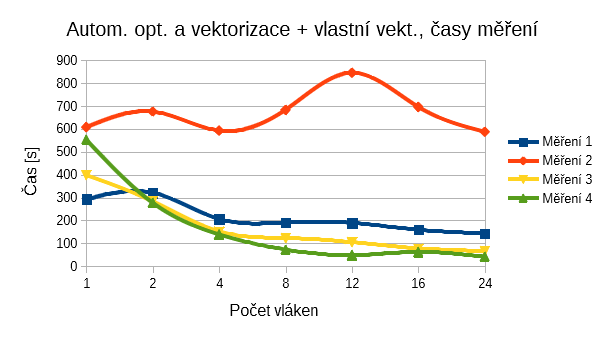
\includegraphics[width=12cm]{images/sdruzene/openmp/mantime.png}
    \caption{Výsledky měření} 
  \end{center}
\end{figure}

Paralelizace varianty č. 3 zrychlila výpočet až 13${\times}$. 
Naměřené výsledky ukazují, že efektivnější využití více vláken ve variantě č. 3 se projeví zejména při vyšším počtu částic.
Následují grafy paralelního zrychlení.

\begin{figure}[H]
  \begin{center}
     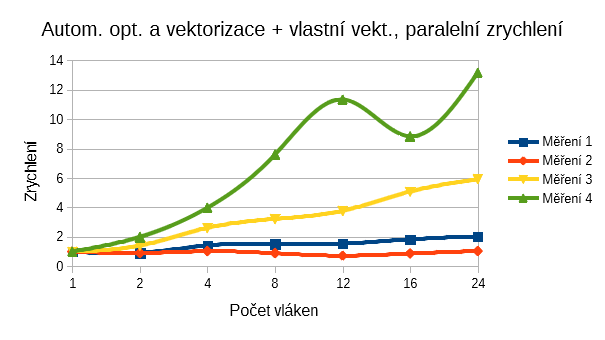
\includegraphics[width=12cm]{images/sdruzene/openmp/manacc.png}
    \caption{Paralelní zrychlení} 
  \end{center}
\end{figure}


% Analýza a hodnocení vlastností dané implementace programu.
\subsection{Porovnání jednotlivých implementací}
První varianta algoritmu, tj. sekvenční s pouze automatickou vektorizací (-O3 -mavx), vyšla jako nejpomalejší ze všech variant.

Vektorizace v dalších dvou variantách přinesla obrovské zrychlení, varianta 2 je oproti variantě 1 až 6${\times}$ rychlejší, varianta 3 oproti variantě 1 přibližně 8${\times}$.

Spuštění varianty 2 na více vláknech přineslo zrychlení až 14${\times}$. Z jednotlivých měření lze usoudit, že zrychlení se zvyšuje i s větším množstvím částic.
Varianta 2 nikdy výpočet nezpomalila, její sekvenční implementace sice je pomalejší než varianta 3, ale v paralelizaci dosahovala většího zrychlení.

Spuštění varianty 3 na více vláknech zrychlilo výpočet až 13,1${\times}$.
Bohužel to v některých případech výpočet i zpomalilo, to přisuzujeme příliš malému množství částic v kombinaci s řežií spojenou s vlákny.
Zrychlení je naopak patrné v měření 3 a 4, kdy se při větším počtu částic výpočet znatelně zrychloval s přibývajícími vlákny.
Varianta 3 také těžila z velmi dobrého sekvenčního času, který předčil i variantu 2 s automatickou opt. a vektorizací.

Dále jsou uvedeny grafy porovnávající variantu 2 a 3, ukazují vliv vektorizace na rychlost výpočtu.

\begin{figure}[H]
  \begin{center}
      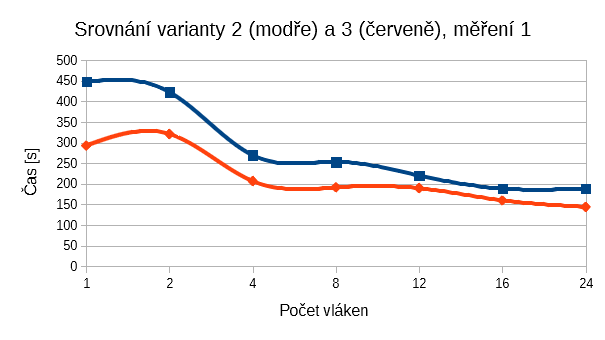
\includegraphics[width=12cm]{images/vs1.png}	
    \caption{Porovnání implementací, měření 1} 
  \end{center}
\end{figure}

\begin{figure}
  \begin{center}
      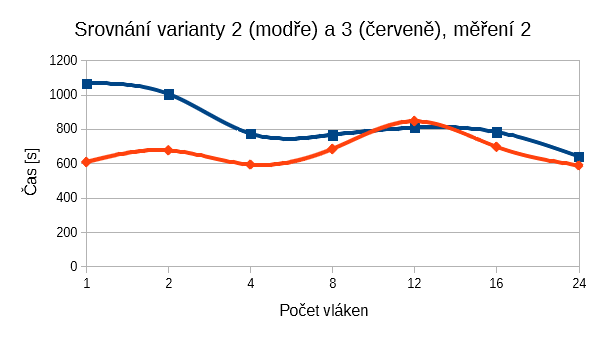
\includegraphics[width=12cm]{images/vs2.png}	
    \caption{Porovnání implementací, měření 2}
  \end{center}
\end{figure}

\begin{figure}
  \begin{center}
      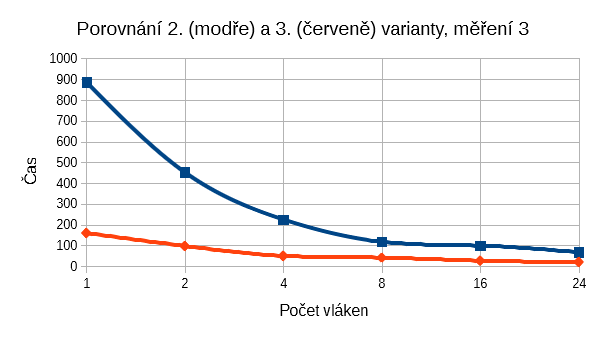
\includegraphics[width=12cm]{images/vs3.png}	
    \caption{Porovnání implementací, měření 3}
  \end{center}
\end{figure}

\begin{figure}
  \begin{center}
      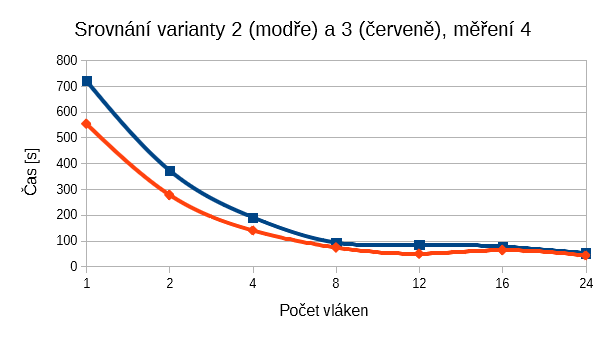
\includegraphics[width=12cm]{images/vs4.png}	
    \caption{Porovnání implementací, měření 4}
  \end{center}
\end{figure}

\section{Naměřené výs\-led\-ky a vyhod\-noce\-ní pro Xeon Phi}
Program pro Xeon Phi byl vytvořen z původního zdrojového kódu jeho kompilací přes icc, tj. kompilátor od Intelu.
Výsledný program je tedy podobný variantě 2 z předchozí sekce, jen jsou automatické optimalizace a vektorizace v režii jiného kompilátoru a přizpůsobené jiné architektuře.

\subsection{Co se měřilo}
Měření proběhlo na stejných datech, pro připomenutí jsou jednotlivá zadání uvedena v následující tabulce.

\begin{center}
\begin{tabular}{c | c | c | c}
\textbf{Měření} & \textbf{Počet částic} & \textbf{Počet kroků sim.} & \textbf{Výpočetní náročnost} \\ \hline \hline
1 & 1024 & 150 000 & 157,284 \\ \hline
2 & 512 & 1 200 000 & 314,571 \\ \hline
3 & 4096 & 15 000 & 251,412 \\ \hline
4 & 8192 & 4 500 & 301.989 \\ \hline
\end{tabular}
\captionof{table}{Zadání měření - pro připomenutí}
\end{center}

\subsection{Vektorizace}
Kompilátor icc provedl automatickou vektorizaci, při které došlo k vektorizaci stejného bloku kódu jako u kompilátoru g++. Vektorizován byl vnitřní cyklus kódu, který počítá to jak se částice navzájem ovlivňují. Vektorizace tohoto úseku kódu má velký vliv na výkonost. Zrychlení je způsobeno tím, že v tomto úseku kódu je třeba počítat vzdálenost 2 částic. V tomto výpočtu figuruje inverzní odmocnina. Díky vektorizaci lze spočítat inverzní odmocninu rychleji a zároveň  lze počítat několik hodnot najednou.

\subsection{Výsledky měření bez vektorizace}
V této sekci jsou uvedeny tabulkově výsledky měření podle počtu vláken pro jednotlivá měření.
Měření je graficky znázorněno v předposlední sekci věnované Xeonu Phi, kde je zároveň i grafické porovnání s variantou s vektorizací a grafy paralelního zrychlení.
\begin{table}[H]
\parbox{.45\linewidth}{
%
% 1. měření
%
\begin{center}
\begin{tabular}{ c | c }
\textbf{Počet vláken} & \textbf{Naměřený čas} \\ \hline \hline 
61 & 158.770535s \\ \hline
122 & 109.994492s \\ \hline
244 & 73.545292s \\ \hline
\end{tabular}
\captionof{table}{Časy 1. měření}
\end{center}
}
\hfill
\parbox{.45\linewidth}{
%
% 2. měření
%
\begin{center}
\begin{tabular}{ c | c }
\textbf{Počet vláken} & \textbf{Naměřený čas} \\ \hline \hline 
61 & 433.739839s \\ \hline
122 & 338.331224s \\ \hline
244 & 311.221709s \\ \hline
\end{tabular}
\captionof{table}{Časy 2. měření}
\end{center}
}
\end{table}

\begin{table}[H]
\parbox{.45\linewidth}{
%
% 3. měření
%
\begin{center}
\begin{tabular}{ c | c }
\textbf{Počet vláken} & \textbf{Naměřený čas} \\ \hline \hline 
61 & 219.587957s \\ \hline
122 & 142.293198s \\ \hline
244 & 80.381402s \\ \hline
\end{tabular}
\captionof{table}{Časy 3. měření}
\end{center}
}
\hfill
\parbox{.45\linewidth}{
%
% 4. měření
%
\begin{center}
\begin{tabular}{ c | c }
\textbf{Počet vláken} & \textbf{Naměřený čas} \\ \hline \hline 
61 & 258.860143s \\ \hline
122 & 167.851305s \\ \hline
244 & 91.632020s \\ \hline
\end{tabular}
\captionof{table}{Časy 4. měření}
\end{center}
}
\end{table}

\subsection{Výsledky měření s vektorizací}
V této sekci jsou výsledky jednotlivých měření s vektorizací.
Grafické znázornění je v následující sekci, včetně grafů paralelního zrychlení.
\begin{table}[H]
\parbox{.45\linewidth}{
%
% 1. měření
%
\begin{center}
\begin{tabular}{ c | c }
\textbf{Počet vláken} & \textbf{Naměřený čas} \\ \hline \hline 
61 & 98.085072s \\ \hline
122 & 116.254455s \\ \hline
244 & 50.155506s \\ \hline
\end{tabular}
\captionof{table}{Časy 1. měření}
\end{center}
}
\hfill
\parbox{.45\linewidth}{
%
% 2. měření
%
\begin{center}
\begin{tabular}{ c | c }
\textbf{Počet vláken} & \textbf{Naměřený čas} \\ \hline \hline 
61 & 393.132266s \\ \hline
122 & 431.340725s \\ \hline
244 & 272.362233s \\ \hline
\end{tabular}
\captionof{table}{Časy 2. měření}
\end{center}
}
\end{table}

\begin{table}[H]
\parbox{.45\linewidth}{
%
% 3. měření
%
\begin{center}
\begin{tabular}{ c | c }
\textbf{Počet vláken} & \textbf{Naměřený čas} \\ \hline \hline 
61 & 30.253954s \\ \hline
122 & 18.628104s \\ \hline
244 & 11.668549s \\ \hline
\end{tabular}
\captionof{table}{Časy 3. měření}
\end{center}
} 
\hfill
%
% 4. měření
%
\parbox{.45\linewidth}{
\begin{center}
\begin{tabular}{ c | c }
\textbf{Počet vláken} & \textbf{Naměřený čas} \\ \hline \hline 
61 & 28.133410s \\ \hline
122 & 17.696219s \\ \hline
244 & 11.387652s \\ \hline
\end{tabular}
\captionof{table}{Časy 4. měření}
\end{center}}
\end{table}

\subsection{Grafické znázornění výsledků měření a paralelního zrychlení}
V této sekci jsou do grafů vyneseny časy z jednotlivých měření pro Xeon Phi.
Poté následují grafy paralelního zrychlení pro obě varianty.
K výpočtu paralelního zrychlení byly použity sekvenční časy varianty 2 z měření pro klasické procesory,
což byla verze s automatickými optimalizacemi a vektorizací provedené kompilátorem g++.
%
% Bez vektorizace - časy
%
\begin{figure}[H]
  \begin{center}
      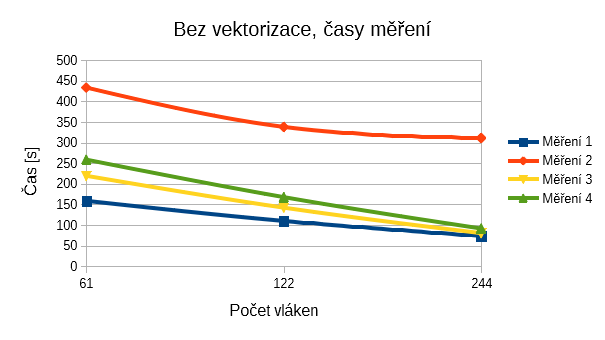
\includegraphics[width=12cm]{images/sdruzene/phi/novectime.png}
    \caption{Výsledky měření bez vektorizace}
  \end{center}
\end{figure}
%
% Bez vektorizace - zrychlení
%
\begin{figure}[H]
  \begin{center}
      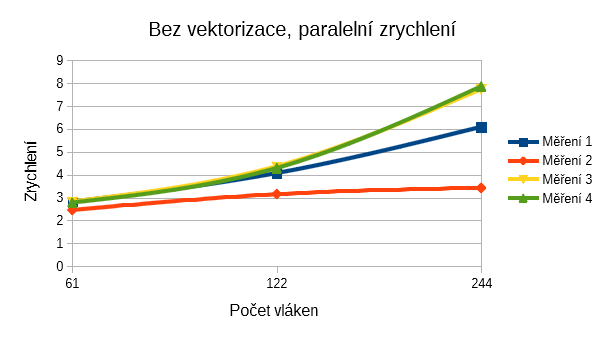
\includegraphics[width=12cm]{images/sdruzene/phi/novecacc.png}	
    \caption{Paralelní zrychlení bez vektorizace}
  \end{center}
\end{figure}
%
% Vektorizace - časy
%
\begin{figure}[H]
  \begin{center}
      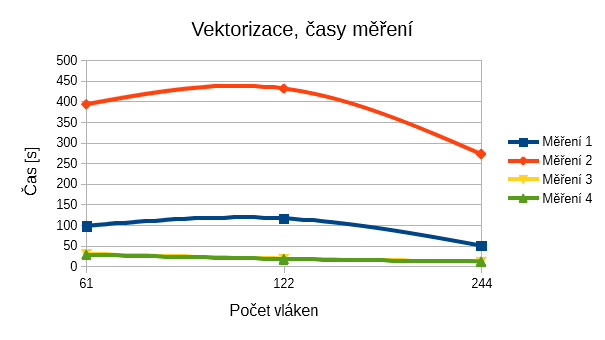
\includegraphics[width=12cm]{images/sdruzene/phi/vectime.png}	
    \caption{Výsledky měření s vektorizací}
  \end{center}
\end{figure}
%
% Vektorizace - zrychlení
%
\begin{figure}[H]
  \begin{center}
      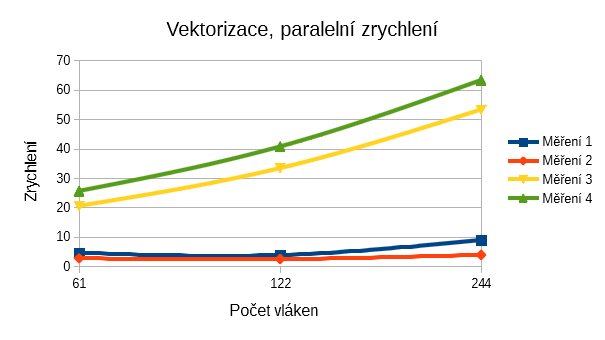
\includegraphics[width=12cm]{images/sdruzene/phi/vecacc.png}	
    \caption{Paralelní zrychlení s vektorizací}
  \end{center}
\end{figure}

\subsection{Vyhodnocení měření}
Ve všech měřeních byl výpočet na Xeonu Phi rychlejší než výpočet provedený na klasických procesorech.
O kolik rychlejší pak záleželo na vektorizaci.
Bez vektorizace dosahovalo zrychlení hodnot až 7,8 v měření č. 4.
S vektorizací bylo dosaženo zrychlení až 63 v měření č. 4.
Lineárního zrychlení dosaženo nebylo.

Zrychlení v měření 1 a 2 v obou variantách dosahovalo znatelně nižších hodnot,
program bez vektorizace byl při některých počtech vláken dokonce rychlejší než varianta s vektorizací.

V měřeních 3 a 4 se naopak hodně ukázala síla vektorizace, kdy zrychlení dosahovalo řádově několika desítek, naproti tomu varianta bez vektorizace pouze v řádu jednotek.

Celkově dopadlo měření podle očekávání.
Kompilátor provedl vektorizaci podobným způsobem jako kompilátor pro klasické procesory, algoritmus ovšem dokázal zužitkovat všech 244 vláken Xeonu Phi a čas výpočtu simulace tak byl výrazně nižší.

\section{Naměřené výs\-led\-ky a vyhod\-noce\-ní pro CUDA}
Implementace pomocí CUDa vycházela z původního sekvenčního algoritmu.
Paralelizace byla provedena jiným způsobem, než v předchozích implementacích pro Xeon Phi a klasické procesory.

\subsection{Popis implementace}
V této sekci je popis implementace za použití technologie CUDA.

Zparalelizován byl vnější cyklus výpočtu nových pozic částic tak,
aby každé vlákno dostalo svou jednu částici a
pro tuto částici vypočetlo zrychlení
(vnitřní cyklus simulace - ten, který se prováděl paralelně v implementacích pro Xeon Phi a klasické procesory).
Důvodem změny paralelizovaného cyklu byla omezená velikost sdílené paměti multiprocesoru,
pomalejší čtení z globální paměti a nutnost paralelní redukce (případně i nad globální paměti) jednotlivých zrychlení, resp. vektorů zrychlení.

Co se týče využití globální paměti, v té jsou uloženy souřadnice částic jako vektor typu float4 (x, y, z, hmotnost) a rychlosti částic jako typ float4 (vx, vy, vz, 0).
Důvod volby typu float4 je v čtení všech informací o částici v jednom jediném čtení z globální paměti a čtení z paměti po 128B.
Tato úprava vyžadovala vytvořit převodník mezi formátem několika za sebou jdoucích lineárních polích (jednotlivě pro x, y, z, atd.) do float4 (x,y,z,m) a (vx, vy, vz, 0).

Sdílená paměť se využívá jako cache pro částice z globální paměti.
Každé vlákno ve svém bloku přečte částici z globální paměti na indexu vypočteném z indexu daného vlákna a sub-bloku.
Sub-blok značí aktuální podmnožinu částic, jejichž vliv se v aktuální iteraci připočítává k částici vlákna.
Dále částici uloží do sdílené paměti na indexu rovném indexu vlákna.
Poté, co každé vlákno bloku toto čtení a uložení provede, začne každé vlákno počítat vlivy ostatních částic na svou přidruženou částici,
přičemž informace o ostatních částicích bere právě z rychlejší sdílené paměti, nikoliv z globální.

Čtení/zápis z/do globální paměti je tedy nutný v každém jednom vlákně v každém kroku simulace,
ale díky využití typu float4 a sdílené paměti by měla být doba přístupu a počet přístupů do globální paměti výrazně nižší.

Vizualizace řešení je stejná jako v předchozích variantách
- přes gnuplot (program vytvoří zdrojový kód pro gnuplot, vygenerovat graf je potřeba ručně).
Dále je možné vizualizovat přímo za běhu simulace přes knihovnu CImg, kdy je ale celkem velká režie v samotném vykreslování a přenosu dat z GPU na CPU.

\subsection{Nastavení kompilátoru}
Ke kompilaci byl použit kompilátor g++ a nvcc. za zmínku stojí využití přepínače -O3, tedy optimalizace.
OpenMP bylo přilinkováno kvůli měření času (ten byl měřen jak přes cudaEvent, tak přes omp\_get\_wtime()).

Příkazy pro kompilaci pro celý program byly následující:
\begin{verbatim}
g++ ./generator/ioproc.cpp -c -o ioproc.o;
g++ ./generator/SimConfig.cpp -c -o SimConfig.o
nvcc -O3 ./main.cu -c -o main.o -Xcompiler -fopenmp

nvcc -O3 ioproc.o SimConfig.o main.o -o \
  simulator -Xcompiler -fopenmp -lcuda -lcudart -lgomp
\end{verbatim}

\subsection{Měřené instance}
Měření proběhlo na stejných datech jako pro Xeon Phi a vektorizované implementace pro klasické procesory.
Pro připomenutí jsou jednotlivá zadání uvedena v následující tabulce.

\begin{center}
\begin{tabular}{c | c | c | c}
\textbf{Měření} & \textbf{Počet částic} & \textbf{Počet kroků sim.} & \textbf{Výpočetní náročnost} \\ \hline \hline
1 & 1024 & 150 000 & 157,284 \\ \hline
2 & 512 & 1 200 000 & 314,571 \\ \hline
3 & 4096 & 15 000 & 251,412 \\ \hline
4 & 8192 & 4 500 & 301.989 \\ \hline
\end{tabular}
\captionof{table}{Zadání jednotlivých měření}
\end{center}

\subsection{Konfigurace bloků a vláken}
Byly zvoleny celkem 3 konfigurace bloků a vláken.

První konfigurace měla přiřadit co možná nejvíc vláken každému jednotlivému bloku, počet bloků se poté dopočítal.
Počet vláken na 1 blok jsme nastavili na polovinu maximálního počtu, co dovolovalo zařízení.
Volba poloviny max. počtu je kvůli dalším HW omezením - při vyšších počtech vláken na blok nebylo dost registrů apod.

Druhá konfigurace měla každému dostupnému procesoru přiřadit právě jeden blok, počet vláken na blok se následně dopočítal.
Tato konfigurace má nevýhodu v počtu vláken - může vznikout blok o malém počtu vláken, resp. warp s několika málo vlákny.
Další riziko bylo v přetečení počtu vláken v posledním bloku - na každé vlákno nemusela vyjít částice.
Tento problém byl vyřešen přes podmínku a dopočet horní hranice, s důsledkem možného dělení warpu.

Cílem třetí konfigurace bylo rozdělit práci mezi bloky v násobcích maximálního počtu vláken v jednom warpu.
Tj. počet vláken na blok byl daný, počet bloků se dopočítal.

\subsection{Výsledky měření}


\subsection{Vyhodnocení}



\end{document}
